\documentclass{article}

\usepackage{graphicx}
\usepackage{tikz}
\usepackage{tikzsymbols}
\usetikzlibrary{calc,patterns,shapes.geometric}
\pagestyle{empty}
\usepackage[margin=0pt]{geometry}
\geometry{papersize={14in,12in}}

\def\centerarc[#1](#2)(#3:#4:#5){\draw[#1] ($(#2)+({#5*cos(#3)},{#5*sin(#3)})$) arc (#3:#4:#5);}

\begin{document}
	\begin{figure}
		\centering
		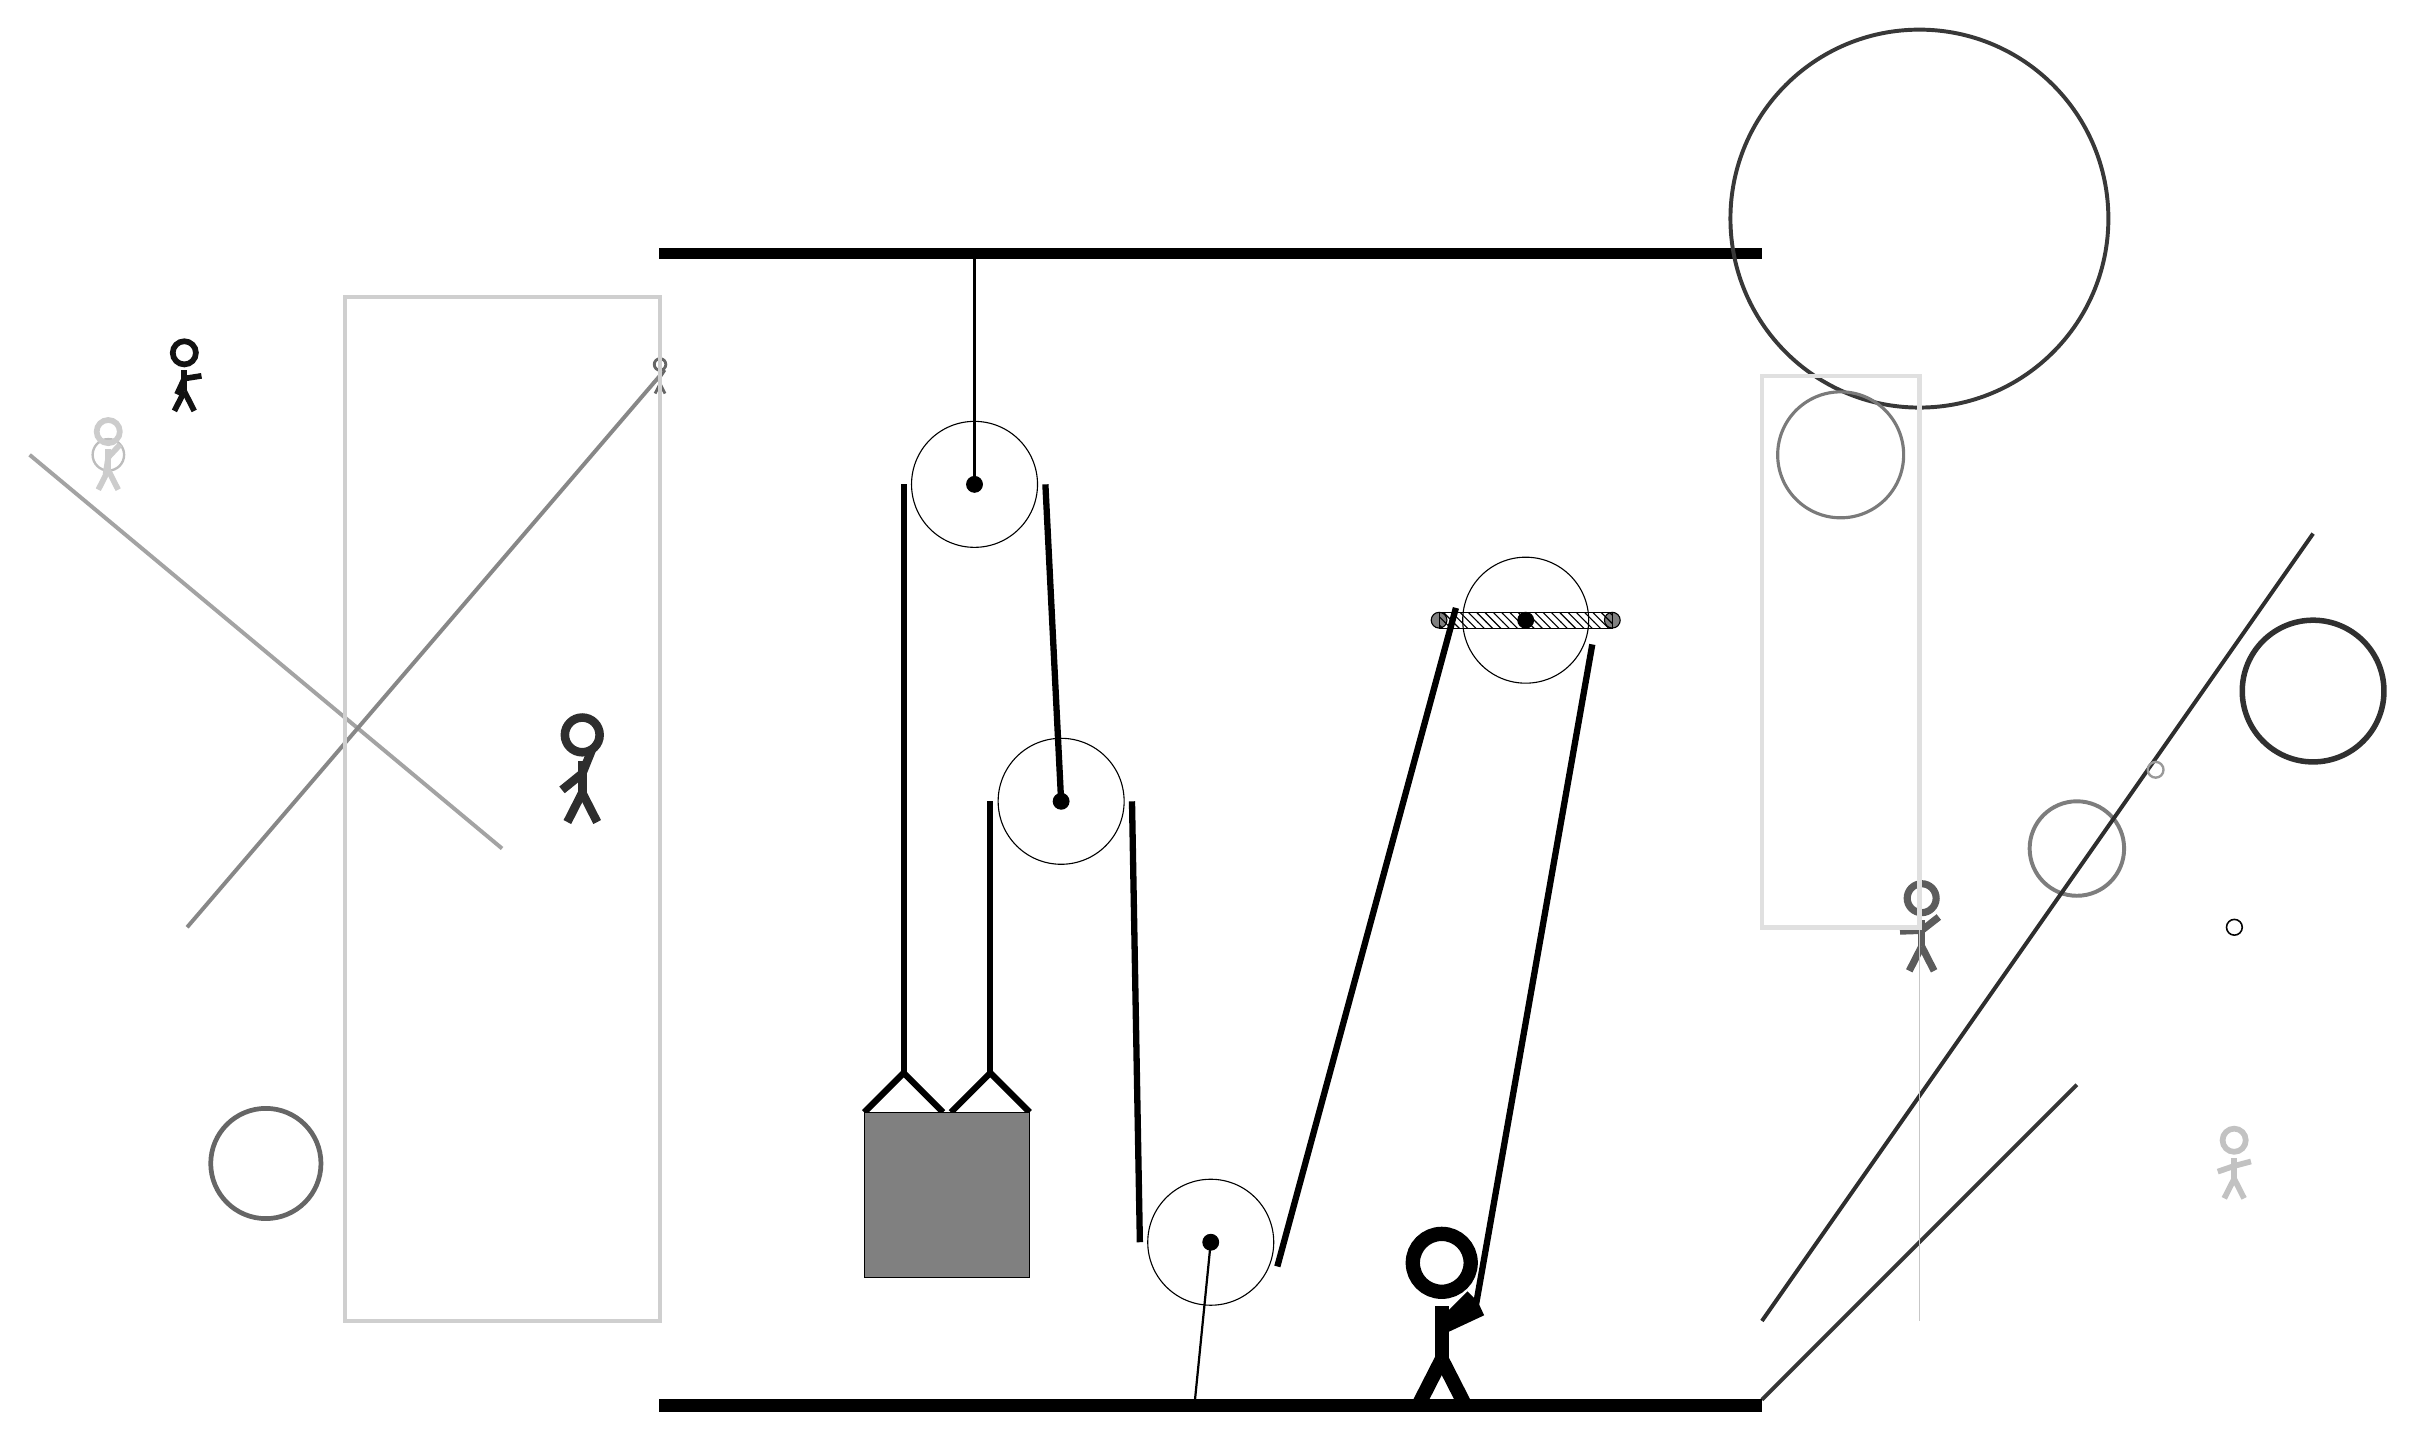
\begin{tikzpicture}
			%%%%% START %%%%%
			
			\draw[fill=black] (-2, 11.5) rectangle (12, 11.625);
			
			\draw (2, 8.625) circle (0.8);
			\draw[fill=black] (2, 8.625) circle (0.1);
			\draw[thick] (2, 8.625) -- (2, 11.5);
			
			\draw (3.1, 4.6) circle (0.8);
			\draw[fill=black] (3.1, 4.6) circle (0.1);
			
			\draw (5, -1) circle (0.8);
			\draw[fill=black] (5, -1) circle (0.1);
			\draw[thick] (5, -1) -- (4.8, -3);
			
			\draw (9, 6.9) circle (0.8);
			\draw[fill=black] (9, 6.9) circle (0.1);
			\draw[fill=black!50] (7.9, 6.9) circle (0.1);
			\draw[fill=black!50] (10.1, 6.9) circle (0.1);
			\draw[pattern=north west lines, pattern color=black] (7.9, 7.0) rectangle (10.1, 6.8);
			
			\draw[line width = 0.8mm]  (0.6, 0.65) -- (1.1, 1.15) -- (1.6, 0.65);
			\draw[line width = 0.8mm]  (1.7, 0.65) -- (2.2, 1.15) -- (2.7, 0.65);
			\draw[fill=black!50] (0.6, 0.65) rectangle (2.7, -1.45);
			
			\node[line width=0.6mm, color=black!60] at (-2, 10) {\Strichmaxerl[2][39][56]};
			
			\node[line width=0.4mm, color=black!24] at (18, 0) {\Strichmaxerl[4][19][15]};
			\draw[line width=0.5mm, color=black!79](16, 1) -- (12, -3);
			\draw[line width=0.5mm, color=black!36](-4, 4) -- (-10, 9);
			\draw [line width=0.5mm, color=black!51](16, 4) circle (0.6);
			\draw[line width=0.5mm, color=black!82](12, -2) -- (19, 8);
			
			\node[line width=0.3mm, color=black!64] at (14, 3) {\Strichmaxerl[5][2][38]};
			\draw[line width=0.5mm, color=black!47](-2, 10) -- (-8, 3);
			\draw [line width=0.3mm, color=black!26](-9, 9) circle (0.2);
			
			\draw [line width=0.6mm, color=black!60](-7, 0) circle (0.7);
			
			\draw [line width=0.5mm, color=black!78](14, 12) circle (2.4);
			
			\node[line width=0.5mm, color=black!20] at (-9, 9) {\Strichmaxerl[4][81][47]};
			\draw [line width=0.3mm, color=black!40](17, 5) circle (0.1);
			
			\node[line width=0.3mm, color=black!93] at (-8, 10) {\Strichmaxerl[4][65][9]};
			\draw[line width=0.2mm, color=black!22] (14, -2) rectangle (14, 6);
			\node[line width=0.7mm, color=black!82] at (-3, 5) {\Strichmaxerl[6][39][68]};
			
			\draw[line width=0.5mm, color=black!19] (-2, -2) rectangle (-6, 11);
			\draw [line width=0.2mm, color=black!99](18, 3) circle (0.1);
			\draw[line width=0.6mm, color=black!12] (14, 3) rectangle (12, 10);
			\draw [line width=0.7mm, color=black!81](19, 6) circle (0.9);
			\draw [line width=0.4mm, color=black!52](13, 9) circle (0.8);
			
			
			\draw[line width = 0.8mm] (1.1, 8.625) -- (1.1, 1.15);
			\centerarc[line width = 0.8mm](2, 8.625)(0:180:0.9);
			\draw[line width = 0.8mm] (2.9, 8.625) -- (3.1, 4.6);
			\draw[line width = 0.8mm] (2.2, 4.6) -- (2.2, 1.15);
			\centerarc[line width = 0.8mm](3.1, 4.6)(0:180:0.9);
			\draw[line width = 0.8mm] (4.0, 4.6) -- (4.1, -1);
			\centerarc[line width = 0.8mm](5, -1)(180:340:0.9);
			\draw[line width=0.8mm](5.8457, -1.3078) -- (8.1137, 7.0562);
			\centerarc[line width = 0.8mm](9, 6.9)(-20:170:0.9);
			\draw[line width=0.8mm](9.8457, 6.5922) --  (8.35, -1.9);
			
			\node at (8, -2) {\Strichmaxerl[10][225][25]};
			
			\draw[fill=black] (-2, -3) rectangle (12, -3.15);
			
			%%%%% END %%%%%
		\end{tikzpicture}
	\end{figure}	
\end{document}